 \documentclass[../Main.tex]{subfiles}
\begin{document}

Nowadays there are plenty of free open-source tools for NN purposes and its number is increasing rapidly with the popularity of ML. The development process of prototyping and training neural networks, implementing mobile application or server is full of nuances. Thus, it is  important to choose up-to-date technologies with well-prepared documentation and active communities, which can help to overcome obstacles. Set of tools selected for this work, fulfills these criteria and allows smooth work, instead of struggling with implementation or configuration.

\subsection{Neural Network}

    \subsubsection{PyTorch}
    \textbf{PyTorch} is an open-source machine learning library created by Facebook and widely used in the field of computer vision. Released in 2016 \cite{pytorch} quickly gained popularity among researchers and developers. PyTorch is not an another Python binding into a C++ framework, but it uses core Python concepts like structures, classes or conditions, so integrates easily with the rest of Python ecosystem. Torch libraries provide all necessary tools for developing and training neural networks based on deep learning models. PyTorch also delivers various neural network models, already implemented and ready to use, which is handy during implementation process presented in this paper.
    
    The main features of this package are:
    \begin{itemize}
        \item Strong \textbf{GPU and TPU acceleration} during computation of tensors
        \item Interactive debugging 
        \item Workflow similar to Python’s scientific computing library (Numpy)
        \item Neural networks built on a tape-based \textbf{autograd system}
    \end{itemize}
    
    Picking out PyTorch instead of TensorFlow (the main alternative) comes with several reasons. Firstly, TensorFlow was becoming more and more complex for machine learning beginners. Whereas PyTorch is based on basic and familiar programming paradigms. The new version of TF (2.0) seems to solve this issue. Anyway, it was released recently and in many opinions is still unstable. Moreover, the documentation is also pretty straightforward and helpful for newcomers. And finally, Pytorch is highly-configurable and is more popular among researchers comparing to developers who don’t need complex architecture or special layer operations. So many experimental projects are build on this package. Including the ones adopted for this paper. 
    
    \subsubsection{CUDA}
    CUDA (Compute Unified Device Architecture) is a parallel computing platform and programming model created by NVIDIA \cite{cudatoolkit}. CUDA allows using equivalent CPU functions for maximum use of GPUs and accelerated programs. It enables training models on GPU with a shorter period of time and allows high floating-point computing performance. Frameworks like PyTorch relay on CUDA for their GPU support. NVIDIA also created CUDA Toolkit, which includes libraries, debugging and optimization tools. There are two key libraries intended for deep learning: 
    \begin{itemize}
        \item CuDNN - the most popular for deep neutral network computations and mostly used in open-source frameworks
        \item TensorRT - the high-performance inference optimizer and runtime
    \end{itemize}
    
    There is possibility to use signal processing and math libraries and in case, writing own low-level CUDA program in C or C++. 

    \subsubsection{OpenCV}
    Open Source Computer Vision Library is an open-source package developed by Intel. Its common use cases are computer vision and machine learning software \cite{opencvdocs}. OpenCV includes tons of computer vision algorithms for detecting and recognizing elements, identifying objects and processing images. Although it is written in C++, OpenCV has solid Python bindings and provides support for ML libraries such as PyTorch. With OpenCV programmers can process images and videos to detect objects, apply filters, analyze structure or perform reconstruction. 
    
    
\subsection{Environment}
    \subsubsection{Google Colab}
    Google Colaboratory is a Google Research product, which allows developers to write and execute Python code through their browser. This tool us useful especially with deep learning tasks. It is a hosted Jupyter notebook, requires no setup and has powerful free version, which gives free access to Google computing resources such as GPUs and TPUs. 
    Google Colab offers non-complicated integration with Github. Notebooks can be hosted on Google Drive or pulled from version control system. Datasets and output files can be automatically saved on personal account storge. User can manage different session and runtimes which enable training and testing different ML models in the same time.
    All these features are accessible in interactive model based on IPython - an improved shell and read–eval–print loop (REPL) for Python. REPL is a simple interactive computer programming environment that takes single user inputs, executes them, and returns the result to the user; a program written in a REPL environment is executed piece-wise.
    Besides many features offered by Colab, it also has a special version for students, which is the main reason why I selected this product for my work. 

    \subsubsection{Google Cloud}
    Google Cloud Storage is a data storage solution. It provides a durable, future-proof platform, with nice performance, option to scale and affordable pricing, that is designed to help researchers businesses of any size. Hosting websites, APIs or servers is fast and simple with Google Cloud, so I decided to use it for testing purposes. Cloud comes with detailed documentation and ready-to-use templates, which makes hosting process rather straightforward. 
    Following elements had to be stored on hosting service in order to provide seamless mobile-server-CNN flow:
    \begin{itemize}
        \item Python packages including Pytorch
        \item Graphic card drivers with CUDA support
        \item Repositories from Github
        \item Datasets used for testing 
        \item Neural Network models
        \item Server and configuration files
    \end{itemize}
    
    \subsubsection{Docker}
    Using OS level virtualization, Docker allows to create containers where we can put our program and all its dependencies. The can be multiple containers managed easily using command line or one of the GUI clients, like \textit{Kitematic}. Docker containers are separated from each other so there is no risk to do any harm to other containers or hosts. Docker containers allow us to \textit{pack up all configuration setup} and deploy on dedicated machines or on dedicated environment. Docker gives the possibility to define whole building process in single file called \textit{Dockerfile}. During container building we can copy files from local drive, download programs from the Internet or run bash scripts. In this project Docker was used to deploy the model, the server, graphic card drivers, configuration files and all other dependencies into single container. After building, container was converted into image and uploaded to the \textit{Dockerhub} - an open docker images library.
    
    
\subsection{Server}
    Client-server communication is divided into two parts: image uploading and transferring image-related specification data. For all operations micro-server based on Flask was implemented. Its segments are written in Python and based on projects developed by open-source Flask communities.

    \subsubsection{Flask}
    Flask is a \textbf{micro-framework} with some dependencies to external Python libraries, which provides tools and technologies helpful during building and hosting small web applications \cite{flaskdocs}. It could be used for developing web pages, blogs or a simple REST servers. Technically, Flask is based on:
    \begin{itemize}
    \item Werkzeug WSGI (Web Server Gateway Interface is a popular specification for a universal interface between the  server and the web app) - toolkit which implements requests-response objects, and some service functions
    \item Jinja2 template engine - template system helpful with rendering dynamic web pages
    \end{itemize}
    
    Flask by default does not support any database handling, extensive visual templates or validations. It is lightweight and designed to do not perform any complicated tasks. Flask server running in the background is usually responsible for:
    \begin{itemize}
        \item Receiving HTTP requests
        \item Encoding or decoding data
        \item Authenticating and authorizing users
        \item Sending confirmation response
        \item And especially in this project case - performing predictions using CNN models
    \end{itemize}
    
    It is always necessary to write simple Flask client in order to test connection to the server.

    \subsubsection{Typical server flow}
    Typical client-server flow with mobile app and API calls is depicted in Figure \ref{fig:server-flow} \\
    
    \begin{figure}[ht]
        \centering
        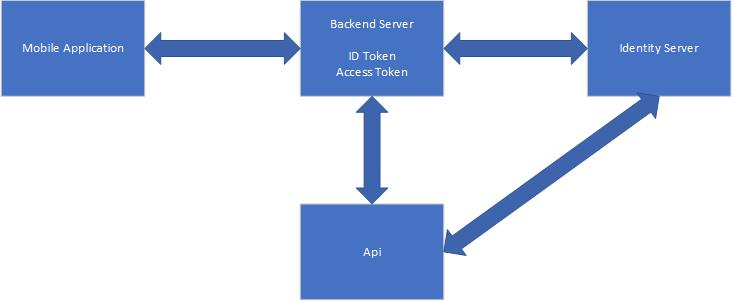
\includegraphics[width=0.7\textwidth]{Images/03_todo.jpg}
        \caption{Client-server flow}
            \label{fig:server-flow}
    \end{figure}


\subsection{Mobile Application}
    This part describes the technologies selected for development of mobile application - the final product of this project.
    
    \subsubsection{Ionic}
    Ionic is an open-source SDK for hybrid mobile app development created in 2013 having more than 5 million apps built using it \cite{ionic}. Current versions are re-built as a set of Web Components, allowing the user to choose any user interface framework, such as Angular, React or Vue.js. It is basically an npm module, requiring Node.js installed to function as part of a large JavaScript ecosystem.Ionic provides tools and services for developing hybrid mobile, desktop, and progressive web apps based on modern web development technologies and practices, using Web technologies like CSS, HTML5, and Sass. Basically, it allows web developers to create web pages that are run inside a device’s browser instance called WebView. WebView may come as a plugin, and it’s essentially an application component that renders web pages and displays them as a native application.
    
    Web Views offer many built-in HTML5 APIs for hardware functionality such as cameras, sensors, GPS, speakers, and Bluetooth, but sometimes it may also be necessary to access platform-specific hardware APIs. In Ionic apps, hardware APIs can be accessed through a bridge layer, typically by using native plugins which expose JavaScript APIs what is presented on \ref{fig:ionic-flow}.
    
    \begin{figure}[ht]
        \centering
        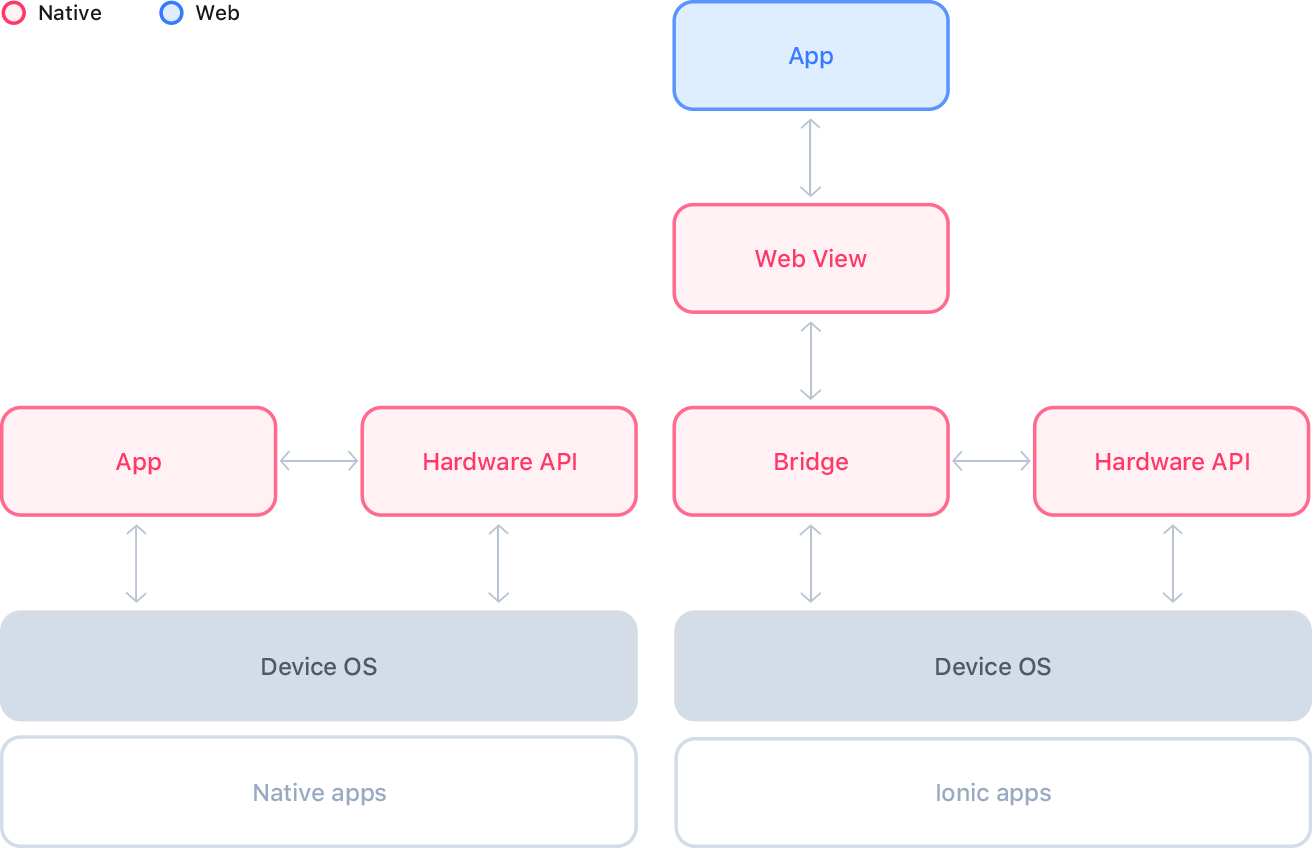
\includegraphics[width=0.6\textwidth]{Images/03_ionic_webview.png}
        \caption{Ionic Web View flow}
            \label{fig:ionic-flow}
    \end{figure}
    
    Nowadays there are several frameworks that allow us to create mobile applications for both Android and iOS simultaneously, eg. Flutter and Xamarin. However, Ionic has several features making it the first choice for multi-platform app:
    
    \begin{itemize}
        \item Comprehensive documentation
        \item An extensive choice of UI elements and quick prototyping
        \item Strong community
        \item Testing convenience using standard browser
        \item Ready-to-use implementation of sensors and app templates
    \end{itemize}
    
    \subsubsection{React}
    Ionic Application can be written in Vanillia JS or in any supported framework. I decided to use ReactJS in order to provide seamless user experience and decent performance.
    
    ReactJS is an open-source, front end, JavaScript library for building user interfaces or UI components. It has been created by Facebook and is currently maintained by community of individual developers and companies \cite{reactjs}. React, as a declarative framework, makes it simple to create interactive UIs. Declarative views make written code more predictable and easy to debug.
    
    It is called component-based framework, because developers can build encapsulated components that manage their own state, then compose them to make complex UIs. Since component logic is written in JavaScript instead of templates, everyone can easily pass rich data through the app and keep state out of the DOM \cite{reactjs}. 
    
    Another Key React feature is Virtual DOM (Document Object Model). React creates an in-memory data-structure cache, computes the resulting differences, and then updates the browser's displayed DOM efficiently in process called reconciliation. This allows the developer to write code as if the entire page is rendered on each change, while the React libraries only render subcomponents that actually change. This selective rendering provides a major performance boost, because it saves the effort of recalculating the CSS style or layout for the page, and rendering for the entire page.
    
\newpage

\biblio % Needed for referencing to working when compiling individual subfiles - Do not remove
\end{document}

